\cotefile{10}
\scanpage{77}
\mspage{76}
quotient de $\handwritten{\overline}{\handwritten{\underline}{Q}}^{\handwritten{*}}$ par le sous-groupe des unités, donc canoniquement isomorphe à $\handwritten{\underline}{Q}$, par l'isomorphisme
\[
\handwritten{\overline}{\handwritten{\underline}{Q}}^{\handwritten{*}}/\text{unités}\handwritten{\longrightarrow}\handwritten{\underline}{Q}
\]
donnés par la valuation p-adique $v_p$, normalisée par la condition
\[
v_p(p)=1\quad .
\]
\unsure{\rlap{A}L|A|L}'opération de $\deleted{\unsure{\pi|\Pi}_1(\underline{\unsure{\rlap{F}K|K|F|k}}}$ $\operatorname{Gal}(\handwritten{\overline}{\handwritten{\underline}{Q}}_p/\handwritten{\underline}{Q}_p)$ sur ce groupe quotient $Q$ est trivial\unsure{\rlap{i}e|\.{e}|e}, de sorte que $H$ est \handwritten{\uline}{diagonalisable} de groupe des caractères $\handwritten{\underline}{Q}$ :
\[
H=D(\handwritten{\underline}{Q})\quad .
\]
L'augmentation de Tate de $G$ correspond à l'homomorphisme
\[
\handwritten{\underline}{Z}\handwritten{\longrightarrow}\handwritten{\overline}{\handwritten{\underline}{Q}}^{\handwritten{*}},\quad 1\handwritten{\longmapsto}p\quad ,
\]
et l'augmentation induite sur $H$ correspond à l'\handwritten{\uline}{inclusion} canonique
\[
\handwritten{\underline}{Z}\handwritten{\lhook\joinrel\longrightarrow}\handwritten{\underline}{Q}
\]
(grâee à notre choix de la valuation \handwritten{\uline}{normalisée} comme indiqué\unsure{\rlap{i}e|\.{e}|e}).

\unsure{\rlap{8}B|B|8}.2. Il faut maintenant expliciter l'homomorphisme de \unsure{\rlap{e}g|g}erbes
\[
\handwritten{\text{(8\unsure{,|.}2.1)}}\qquad\handwritten{i:}\ \handwritten{\underline}{G}(\handwritten{\underline}{F}_p)\handwritten{\longrightarrow}\handwritten{\underline{\pi}}_p(\handwritten{\underline}{F}_p)

\]
correspondant à l'inclusion
\[
i:\quad \handwritten{\underline}{Q}_p\text{-faisceaux constructibles}\handwritten{\lhook\joinrel\longrightarrow}\operatorname{Fcriso}(\handwritten{\underline}{F}_p)
\]
de 5.2. On a vu que l'image essentielle est exactement égale à la sous-catégorie \inserted{pleine}\handwritten{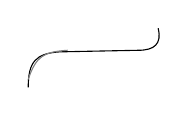
\begin{tikzpicture}[baseline=0cm,x=1cm,y=1cm]\draw[thin] (0,-.35)..controls (0,-.02) and (.1,.08)..(.4,.1)--(1.4,.12)..controls (1.6,.12) and (1.7,.2)..(1.65,.4);\draw[gray,thin] (0,-.25)..controls (.1,.05) and (.2,.1)..(.5,.12);\end{tikzpicture}} $j(\handwritten{\underline}{Q}_p\text{-faisceaux constructibles})$, \deleted{qui est} de sorte que $i$ s'identifie à une\deleted{foncteur} $\handwritten{\unsure{\mathrel{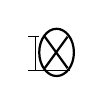
\begin{tikzpicture}[baseline=-.12cm,x=1cm,y=1cm]\draw[thick] (.05,0) ellipse (.22 and .3);\draw[thick] (-.1,-.2)--(.19,.2);\draw[thick] (-.1,.2)--(.19,-.2);\draw[thin] (-.22,-.23)--(-.22,.2);\draw[thin] (-.31,.2)--(-.17,.2);\draw[thin] (-.31,-.23)--(.22,-.23);\end{tikzpicture}}}}$-équivalence de la catégorie des $\handwritten{\underline}{Q}_p$-faisceaux constructibles avec elle-même. On constate alors que l'homomorphisme correspondant sur les liens $\deleted{\unsure{H\ H|H\to H}}$ $G'\handwritten{\longrightarrow}G'$ est l'identité, \deleted{et que} de sorte que $i$ est défini par un torseur sous $G'$, et que ce torseur sous $G'$ peut se décrire ainsi (aurait pu passer à la fin de 7, dans le cas d'un $k$ quelconque ...). On a un homomorphisme canonique
\[
\handwritten{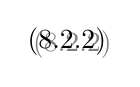
\begin{tikzpicture}[baseline=(dark.base),x=1cm,y=1cm]\node[gray,inner sep=0pt] at (.07,-.04) {$(8.2.2)$};\node[inner sep=0pt] (dark) at (0,0) {$(8.2.2)$};\end{tikzpicture}}\qquad\handwritten{\pi}_1(\handwritten{\underline}{F}_p^{\deleted{\handwritten{\unsure{*|\times}}}})=\overset{\deleted{\handwritten{\unsure{2|*|\times}}}}{\handwritten{\hat}{\handwritten{\underline}{Z}}}\handwritten{\longrightarrow}G'(\handwritten{\underline}{Q}_p),\quad \handwritten{\text{i.e. }(\pi_1(\underline{F}_p))_{\mathbb{Q}_p}\longrightarrow G'}

\]
d'où un \deleted{homomorphi} foncteur
\[
\text{torseurs}^{\deleted{\underline{Q}_p\text{-}}}\text{ sous }(\handwritten{\hat}{\handwritten{\underline}{Z}})_{\handwritten{\underline}{Q}_p}\handwritten{\longrightarrow}\text{torseurs sous }G'\ \deleted{\handwritten{\unsure{\xi|\varepsilon|,|.}}}
\]

